\documentclass[12pt,twoside]{report}
\usepackage[utf8]{inputenc}

\usepackage{graphicx}
\usepackage{ngerman}
\usepackage[a4paper, width=150mm, top=25mm, bottom=25mm, bindingoffset=6mm]{geometry}

\usepackage{fancyhdr}
\pagestyle{fancy} %% there the header is been set up 
\fancyfoot{}
\fancyfoot[LE,RO]{\thepage}
\fancyhead[LE,RO]{\rightmark}
\usepackage{biblatex}
\addbibresource{chapters/references.bib}
\usepackage[colorlinks=true, citecolor=blue, linkcolor=black]{hyperref}


\graphicspath{ {images/} }
\title{
	{Nachweis von Starkregenereignissen in regionalen Klimamodellen}\\
	{\large Wegener Center for Climate and Global Change}\\
	{
\includegraphics{university.jpg}}
}
\author{Lukas Moser}
\date{01.01.10}
\begin{document}
	\maketitle
	\pagestyle{fancy}
	\chapter*{Abstrakt}
	In dieser Arbeit wird evaluiert, wie gut sich globale Klimamodelle wie z.B. MPI-ESM-LR auf regionalen Maßstab skalieren lässt. Dazu werden die Daten von zwei unterschiedlich skalierten regionale Klimamodellen mit Werten aus der Vergangenheit verglichen. Hauptsächlich soll dabei auf Starkregen-Ereignisse wie zum Beispiel Gewitterzellen eingegangen werden. Evaluiert wurden dabei ALP-3 und EUR-11. ALP-3 sind  die Ergebnisse einer Konvektions-erlaubenden Klimasimulation mit dem regionalen Klimamodell CCLM5-0-9, wobei dafür EUR-11 mittels CCLM5-0-9 auf eine Auflösung von 3 km gebracht wurde. EUR-11 sind die Ergebnisse der angetrieben mit CCLM4-8-17, einem Standard-Klimamodell, mit 12.5km Auflösung - damit sind regionale Konvektionszellen nicht simulierbar, da diese sich auf wesentlich kleineren Maßstäben abspielen.\\
Beide regionalen Klimamodelle (ALP-3 und EUR-11) wurden jeweils mit drei unterschiedlichen Datensätzen angetrieben: 
\begin{itemize}
	\item mit Re-Analysedaten der Periode 1996-2005
	\item mit historischen Daten der Klimasimulation MPI-ESM-LR (r2i1p1) aus der Periode 1986-2005
	\item mit Zukunftsdaten der Klimasimulation MPI-ESM-LR und dem Treibhausszenario RCP8.5, dem höchsten der RCP-Szenarios, mit Daten aus der Periode 2090-2099
\end{itemize}

The climate system is complex and high-dimensional, and models are not intended to be isomorphisms of nature [Stainforth et al., 2007]; thus no climate model or downscaling method can be expected to
reproduce all aspects of the system perfectly, and a validation of all aspects would be practically impossible. However, in any given application only a small part of the system will be relevant: specific variables or phenomena, at specific space and time scales in a specific region. A user focused approach to validation must therefore start by identifying the phenomena and scales of interest; with respect to these, it must seek to identify the key strengths and weaknesses of a method. For a given application, it has to give advice whether a method performs well or even better than other methods, and where it is likely to fail. In this way, users can determine whether a particular method is appropriate for their application, and
can compare methods.
	\chapter*{Danksagungen}
	
Ich honoriere den E-OBS Datensatz vom EU-FP6 Projekt UERRA (http://www.uerra.eu) und die Datenprovider im ECA\&D Projekt (https://www.ecad.eu) Cornes, R., G. van der Schrier, E.J.M. van den Besselaar, and P.D. Jones. 2018: An Ensemble Version of the E-OBS Temperature and Precipitation Datasets, J. Geophys. Res. Atmos., 123. doi:10.1029/2017JD028200
\cite[für weitere Informationen siehe][]{eobs}\\
\hfill\\
Ich honoriere den APGD Datensatz vom EURO4M APGD Projekt des Meteoswiss
Dataset DOI: 10.18751/Climate/Griddata/APGD/1.0 Die Dokumentation des Datensatzes findet man unter \cite{apgd}, sowie den dazugehörigen Artikel in der Zeitschrift International journal of climatology \cite[siehe][]{apgd_article}. \cite[für weitere Informationen siehe:][]{meteoswiss}\\
\hfill\\
Ich honoriere das Projekt RStudio \cite{RStudio}, das mir bei der Manipulation und Darstellung der Daten viel geholfen hat.

	\tableofcontents
	
	\chapter{Einführung}
	Das Klimasystem ist ein komplexes und hoch-dimensionales System. Dieses durch ein Modell berechenbar zu machen ist dementsprechend schwierig und bedarf einiger Abstraktionen. Laut Definition (vgl. Stachowiak in \cite{stachowiak}) sollen Modelle nicht alle Attribute des abgebildeten Systems übernehmen, sondern vielmehr eine Vereinfachung dessen sein mit einer kleinst-möglichen und aber notwendig großen Komplexität. Auf Klimamodelle bezogen, bedeutet dies, dass man nicht alle einzelnen Bausteine des Klimas durch das Modell abbilden soll, sondern manche Bausteine durch Parameter und Annäherungen abgebildet werden müssen. Ein globales Klimamodell (GCM) liefert im generellen recht gute Aussagen über die Entwicklung des globalen Klimas, jedoch beruhen diese Ozean-Atmosphären gekoppelten Zirkulationsmodelle, auf einer Parametrisierung der Konvektion, da diese im relativ groben Raster eines GCM nicht simuliert werden kann. Dadurch können grobe Fehler entstehen. (vgl. Stevens \& Bony in \cite{stevensbony}). Jedoch ist aufgrund der Rechenkosten und Rechenzeit eine solche Herangehensweise mit parametrisierter Konvektion im Simulieren großflächiger (globaler) Klimamodelle  unumgänglich. Großflächige Prozesse des Klimas wie z.B. der polare Jet, die nordatlantischen Stürme oder auch die stationären planetaren Wellen werden jedoch in den Modellen simuliert.\\
Viele GCMs bzw. deren Simulationsergebnisse müssen aufgrund der Parametrisierung und auch anderer Probleme wie z.B. der Darstellung der Topographie in niedriger Auflösung korrigiert werden. Dadurch sind diese GCMs eine starke Fehlerquelle in regionalen Klimamodellen (vgl. \cite{woollings_2013}).\\
Um akkurate Aussagen über die regionale Klimaveränderung  basierend auf GCMs zu tätigen, muss das globale Klimamodell auf die entsprechende Region downgescaled werden. Da auf der regionalen Ebene die Ortographie (wie z.B die Alpen), die flache Konvektion, die zur Tiefen-Konvektion wird und die lokalen Kältepools große Auswirkungen auf die Wettererscheinungen haben, müssen diese entweder statistisch parametrisiert oder dynamisch berechnet werden. Diese Vereinfachungen sind auch eine große Fehlerquelle für die regionalen Klimamodelle (vgl. \cite{maraun_2010,casanueva_2013}).\\
%Zudem kommen noch etwaige Rückkopplungen des regionalen Klimas auf das Globale hinzu, was zu einer weiteren Fehlerquelle führen kann. Wie man in der Publikation von Teixera et al.\cite{teixeracardoso} und Chen et al.\cite{chenshuyi} lesen kann hat die flache Konvektion durch ihre starke Rückwirkungen auf die Tiefen-Konvektion auch eine Auswirkung auf das globale Klima, wie es z.B. gut anhand der Tropen und der Madden-Julian Oszillation zu erkennen ist, wo aus flacher Konvektion Tiefen-Konvektoin wird und daraus sich großflächige Wettererscheinungen bilden.
Zudem sollte hier angeführt werden, dass auch die Auflösung von gegenwärtigen Klimamodelle nicht immer ausreichend ist: z.B. können Turbulenzen und andere atmosphärische Mikroprozesse häufig nicht von der derzeitigen Maschenweite der Simulationsgitter vollends erfasst und müssen, um grobe Fehler zu vermeiden, statistisch und dynamisch kombiniert downgescaled werden (vgl. \cite{marauntowards}).\\
Als letzte große Fehlerquelle für regionale- und auch globale Klimamodelle sollte die interne Variabilität des Klimas angeführt werden: Alle externen Klimaeinflüsse wie z.B. der Mensch oder auch vulkanische und astronomische Erscheinungen führen zu einer Klimareaktion, welche von internen Klimafluktuationen überlagert wird. Da diese Klimaeinflüsse nicht modelliert werden können ist es auch nicht möglich ein Klimamodell zu entwickeln, welches nicht von zufälligen Fluktuationen dominiert ist (siehe \cite{maraun_value}, Seite 3).\\
\begin{figure}[h]
	\centering
	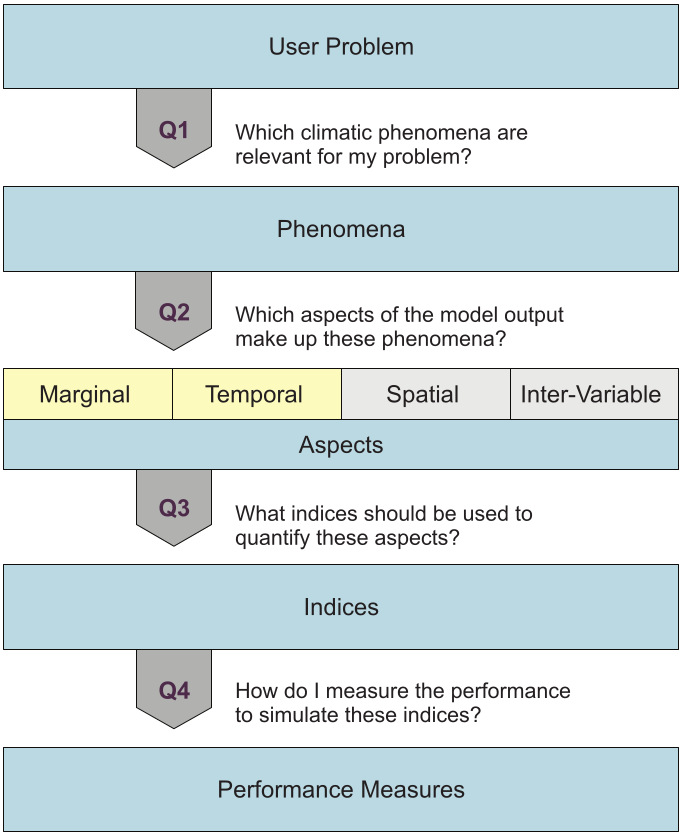
\includegraphics[width=0.5\textwidth]{VALUE.png}
	\caption{Baumstruktur, um eine geeignete Evaluationsmethode zu finden \cite{maraun_value}}
	\label{fig:value}
\end{figure}

Um eine geeignete Evaluierungsmethode zu finden, halte ich mich an die Herangehensweise aus Abb. \ref{fig:value}:
\begin{itemize}
	\item Q1: Starkregenereignisse, und Übereinstimmung von Niederschlagsmustern
	\item Q2:
		\subitem{*} Marginal: Intensität
		\subitem{*} Temporal: Jahreszeit bzw. Dauer der Erscheinungen.
		\subitem{*} Spatial: Gewitterzellen sind auf kleinen Arealen zu finden (in den Alpen)
		\subitem{*} Inter-Variable: Temperatur als Begleiterscheinung bei Gewittern.
	\item Q3: Mittelwert der Niederschläge, 99. Quantile, Jahreszeiten, Temperatur-Niederschlagskorrelation, Übereinstimmung der Verteilungskurven und damit dem BIAS der Kurven, räumliche Übereinstimmung mit den Beobachtungsdaten.
	\item Q4: BIAS und relative Fehler (zu den Beobachtungsdaten)
\end{itemize}

Um nun die beiden regionalen Klimamodelle möglichst allgemein miteinander zu vergleichen werde ich sie über den Mittelwert des Niederschlags, das 99. Quantil über alle zehn Jahre und das 99. Quantil in den vier Jahreszeiten vergleichen. In allen Fällen soll besonders auf die örtliche Verteilung Wert gelegt werden, da dies ein ausschlaggebender Punkt für die Vorhersagekraft regionaler Klimamodelle ist.





	\chapter{Grobe Evaluierung über das Jahresmittel des Niederschlags}
	Um ein Bild von der allgemeinen Übereinstimmung der simulierten Daten mit den tatsächlich beobachteten Daten zu erhalten wird in diesem Kapitel das Jahresmittel der simulierten und beobachteten Daten verglichen. Dadurch erhält man einen Überblick über die geographische Übereinstimmung der Regenzonen und Trockengebiete im abgebildeten Bereich.
\section{Herangehensweise}
\begin{enumerate}
	\item Berechnung des jährlichen Mittelwertes pro Gitterzelle über aller Jahre
	\item Subtraktion dieser Mittelwerte (Simuliert - Beobachtet): Mittelwerte pro Gitterzelle über diese Differenzen; ein Mittel über die gesamten zehn Jahre der Simulationsdaten	
\end{enumerate}
\section{Mittlerer Bias}
In diesem Unterkapitel soll das Verhalten der gemittelten Differenzen aller Datensätze aufgezeigt werden.\\
Wie man gut in den Abbildungen \ref{fig:mean_boxplots} erkennen kann, liegt die Abweichung der Evaluation-Datensätze weit näher bei 0 als die in den Historical-Datensätzen. Des Weiteren ist gut zu erkennen, dass die Abweichung des Datensatzes ALP-3 betrieben mit den Re-Analysedaten (Evaluation) die Beobachtungsdaten gut abbilden und somit im Mittel ein relativ gutes Klimamodell für den Alpenraum darstellt.
Beide Klimamodelle betrieben mit dem GCM MPI-ESM-LR (Hisorical) liefern Ergebnisse, die eine starke Abweichung in positive Richtung aufweist, wobei sie sich nur mehr in der Größe der Ausreißer unterscheiden: Das CCLM5-0-9 hat weitaus stärkere Ausreißer zu den Beobachtungsdaten. Die Abbildungen zeigen, dass im Mittel zwar die Ausreißer des regionalem Klimamodell CCLM5-0-9 im Gegensatz zum CCLM4-8-17 dominieren jedoch sich der mittlere Bias kaum unterscheidet. Im Mittel ist also die Vorhersagequalität der beiden Modelle nahezu identisch. Man kann auch beim Vergleichen der beiden Evaluation-Datensätze mit den beiden Historical-Datensätzen erkennen, dass das globale Klimamodell im Alpenraum den Niederschlag zu stark simuliert, was den ins Positive verschobenen Bias erklärt.\\
Da sich diese Abweichungen nicht über das gesamte Gitter gleich abzeichnen wird in Folge auf die geographische Verteilung der Abweichungen eingegangen.

\begin{figure}[h!]
	\begin{subfigure}{0.49\textwidth}
		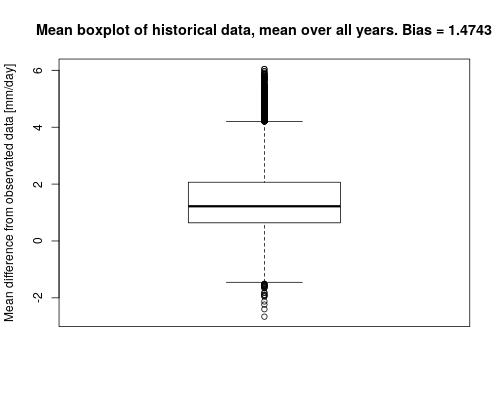
\includegraphics[width=\textwidth]{mean_n/eur_11_mean_historical_boxplot.jpg}
		\caption{Historical, EUR-11}
	\end{subfigure}
	\begin{subfigure}{0.49\textwidth}
		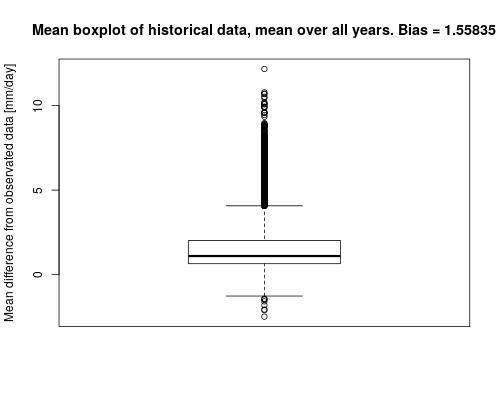
\includegraphics[width=\textwidth]{mean_n/alp3_mean_historical_boxplot.jpg}
		\caption{Historical, ALP-3}
	\end{subfigure}
	\begin{subfigure}{0.49\textwidth}
		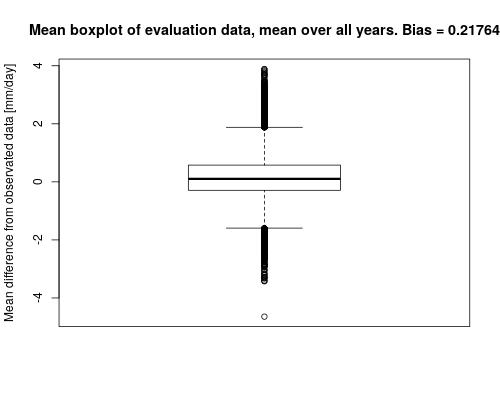
\includegraphics[width=\textwidth]{mean_n/eur_11_mean_evaluation_boxplot.jpg}
		\caption{Evaluation, EUR-11}
	\end{subfigure}
	\begin{subfigure}{0.49\textwidth}
		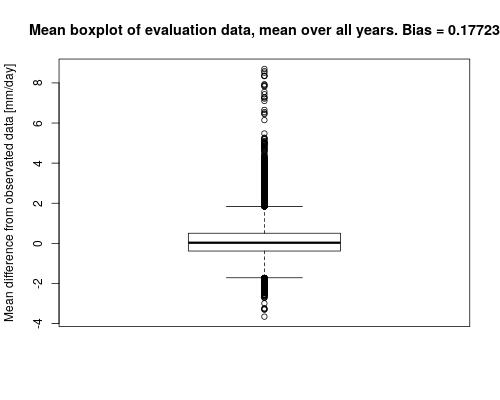
\includegraphics[width=\textwidth]{mean_n/alp3_mean_evaluation_boxplot.jpg}
		\caption{Evaluation, ALP-3}
	\end{subfigure}
	\caption{Box-Plots der Differenzen des jährlichen Mittels des Niederschlags gemittelt über alle Jahre}
	\label{fig:mean_boxplots}
\end{figure}


\begin{figure}[h!]
	\begin{subfigure}{0.49\textwidth}
		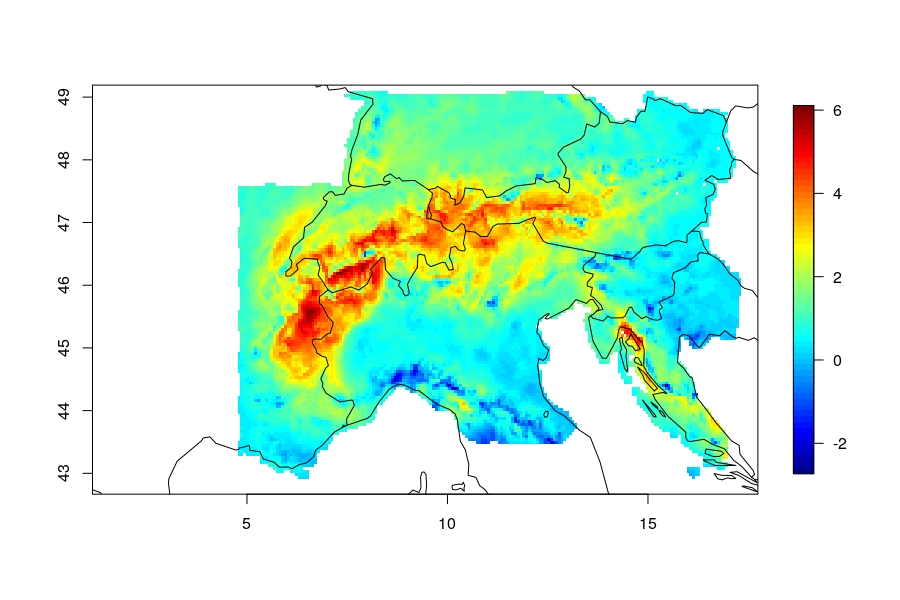
\includegraphics[width=\textwidth]{mean_n/mean_diff_hist_eur11.jpeg}
		\caption{Historical, EUR-11}
	\end{subfigure}
	\begin{subfigure}{0.49\textwidth}
		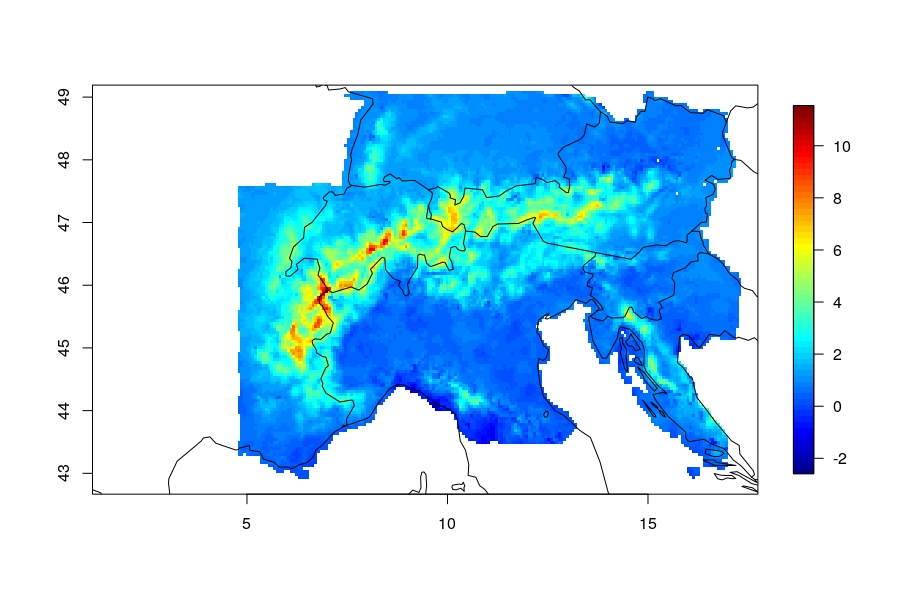
\includegraphics[width=\textwidth]{mean_n/mean_diff_hist_alp3.jpeg}
		\caption{Historical, ALP-3}
	\end{subfigure}
	\begin{subfigure}{0.49\textwidth}
		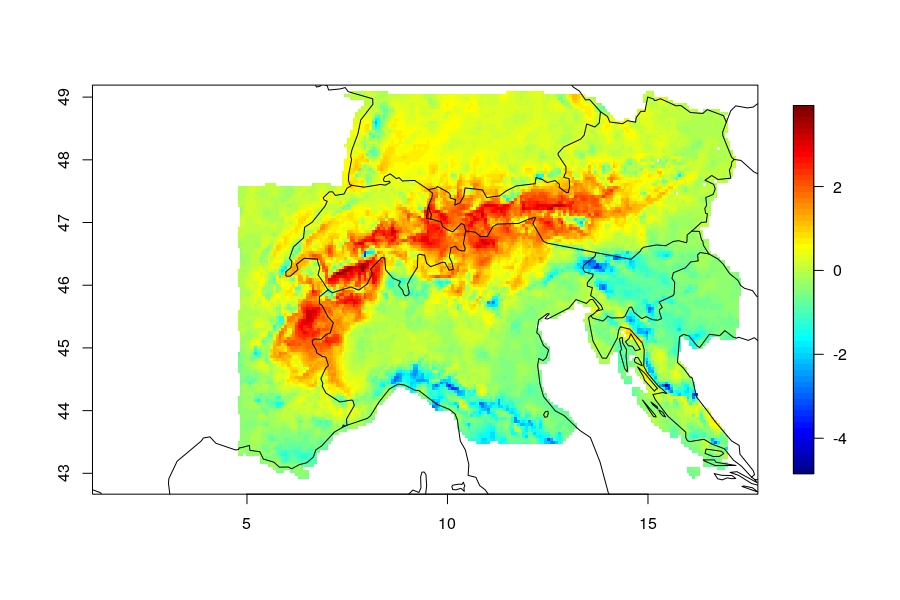
\includegraphics[width=\textwidth]{mean_n/mean_diff_eval_eur11.jpeg}
		\caption{Evaluation, EUR-11}
	\end{subfigure}
	\begin{subfigure}{0.49\textwidth}
		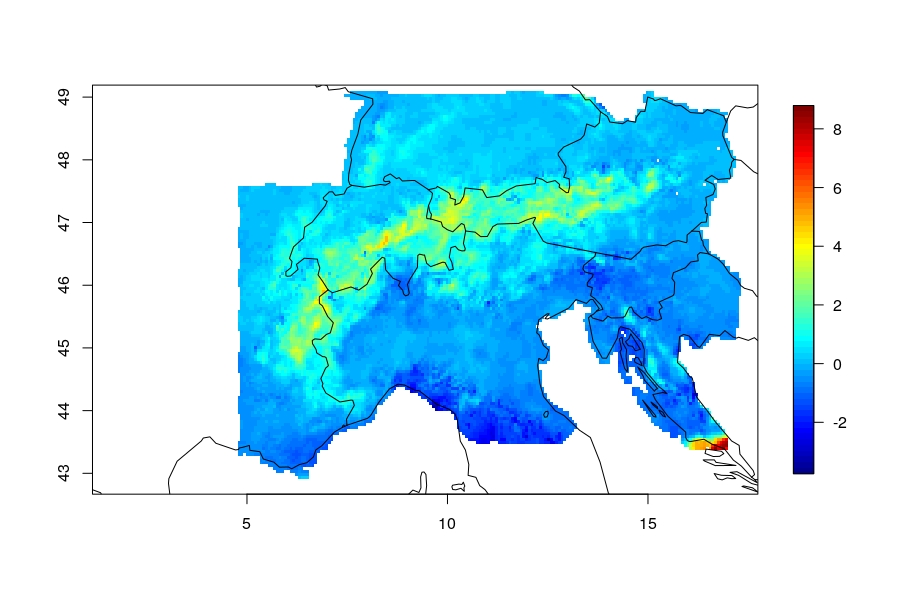
\includegraphics[width=\textwidth]{mean_n/mean_diff_eval_alp3.jpeg}
		\caption{Evaluation, ALP-3}
	\end{subfigure}
	\caption{Geographische Verteilung der Differenzen (Modell-Beobachtungsdaten) vom jährlichen Mittel des Niederschlags [mm/Tag] gemittelt über alle Jahre}
	\label{fig:mean_diff}
\end{figure}

Die geographische Verteilung der Abweichungen wurden in Abb. \ref{fig:mean_diff} für alle Datensätze dargestellt. Man erkennt gut, dass sich die größten Abweichungen an den Gebirgskämmen abzeichnen, über den orthographisch gediegenen Gegenden ist die Abweichung vom Beobachtungsdatensatz relativ gering. Das hat den Grund, dass sich in gebirgigen Gegenden  kleinen Konvektionszellen bilden, die sich zu größeren Regenzellen aufschaukeln können. Das gröber aufgelöste Modell CCLM4-8-17 mit einer Auflösung von ungefähr 15km kann diese Wettererscheinungen nicht modellieren - viele Täler in diesen Gegenden sind schmäler als 15km. Sie sind nur durch die parametrisierte Konvektion darstellbar. Dieses Modell scheint durch sein höheres Alter bereits feiner getuned geworden zu sein als das verglichene CCLM5-0-9: Die Abweichungen überschreiten kaum die 6 mm/Tag, wie auch schon in der Abbildung \ref{fig:mean_boxplots} dargestellt ist.\\
Das feiner aufgelöste regionale Klimamodell CCLM5-0-9 (ALP3) müsste in diesen Gegenden einen klaren Vorteil haben, da die Konvektion dynamisch simuliert wird. Jedoch scheinen die Gleichungen bzw. die einzelnen Module des Modells noch nicht hinreichend abgestimmt (getuned) worden zu sein.\\
Ein im Kapitel \ref{chap:modells} beschriebener negativer Randeffekt des Nestings zeigt sich besonders im Evaluation-Datensatz, wo im Süden Kroatiens ein extremer Ausreißer auszumachen ist, diese Ausreißer zeichnen sich auch im entsprechenden Boxplot ab. (vgl. Abb.\ref{fig:mean_boxplots}). Die größten Abweichungen liegen nahe am Rand vor. Diese werden verursacht durch z.B. zu kleine Bufferzonen zum übergeordneten Modell oder Effekte der zeitlichen und räumlichen Interpolation der GCM - Daten.\\
Beachtenswert ist, dass alle RCMs eine Abweichung ins Positive aufweisen - dies bedeutet, dass mehr Niederschlage simuliert wurde als es tatsächlich gab. Da es sich für beide Klimamodelle betrieben mit GCM und auch den Reanalysedaten so verhält kann es auf eine Schwäche der beiden RCMs zurückgeführt werden. Es muss beachtet werden, dass das CCLM5-0-9 in das gröbere CCLM4-8-17 genested ist. Dadurch zeichnen sich die Abweichungen des gröberen RCMs auch im feinerem ab.

\begin{comment}
\section{Beobachtungen eines Jahres: 2002} \label{section:2002}
Das Jahr 2002 wurde gewählt, da sich in diesem Jahr die stärksten Abweichungen zeigen. In diesem Kapitel soll es darum gehen, die örtliche Verteilung der Differenzen näher zu betrachten. Dazu wurden zunächst die Abweichungen des Jahresmittels bildlich für die beiden Evaluation-Datensätze dargestellt: Abb. \ref{fig:dif_mean_2002}. Wie man erkennen kann, häufen sich Analog zu den Differenzen, gemittelt über alle Jahre die Abweichungen besonders in den gebirgigen Gebieten, in den Ebenen scheint die Übereinstimmung mit den Beobachtungsdaten gut zu sein.\\
\begin{figure}[h]
		\begin{subfigure}{0.49\textwidth}
			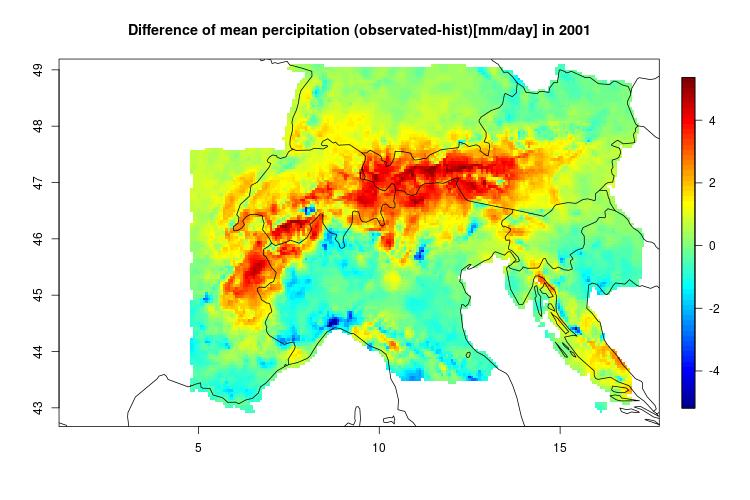
\includegraphics[width=\textwidth]{mean_n/2002dif_mprs_hist-obs.jpg}
			\caption{Historical, EUR-11}
			\label{fig:dif_mean_2002:eur11_hist}
		\end{subfigure}
		\begin{subfigure}{0.49\textwidth}
			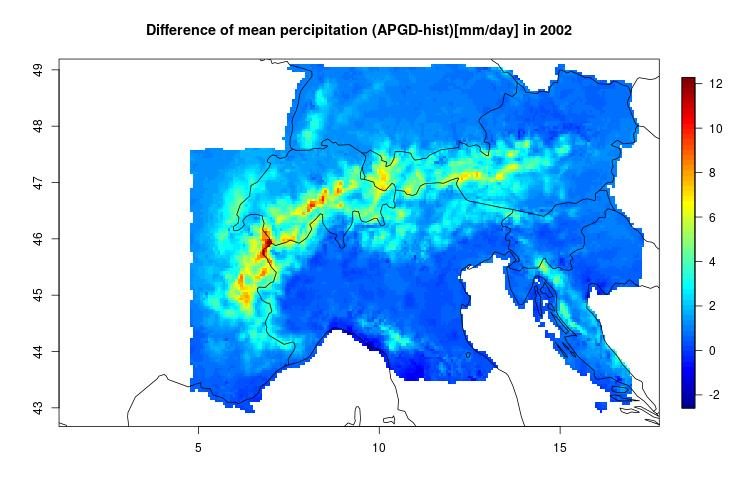
\includegraphics[width=\textwidth]{mean_n/2002dif_mprs_alp3hist-apgd.jpg}
			\caption{Historical, ALP-3}
			\label{fig:dif_mean_2002:alp3_hist}
		\end{subfigure}
		\begin{subfigure}{0.45\textwidth}
			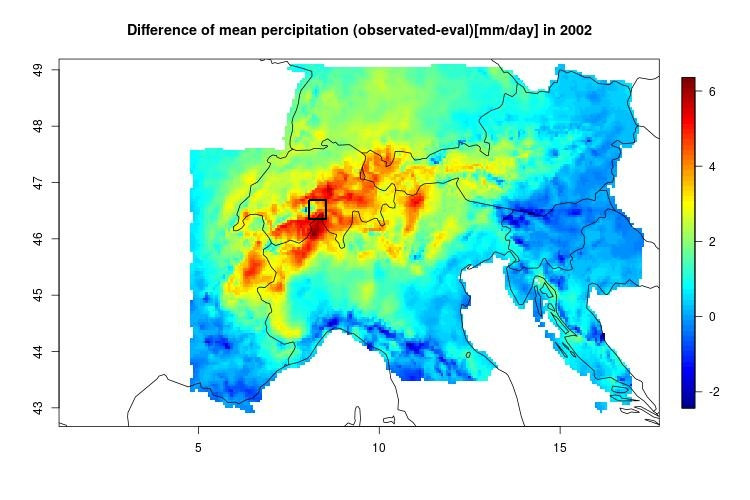
\includegraphics[width=\textwidth]{mean_n/2002dif_mprs_eval-obs.jpg}
			\caption{Evaluation, EUR-11}
			\label{fig:dif_mean_2002:eur11_eval}
		\end{subfigure}
		\begin{subfigure}{0.45\textwidth}
			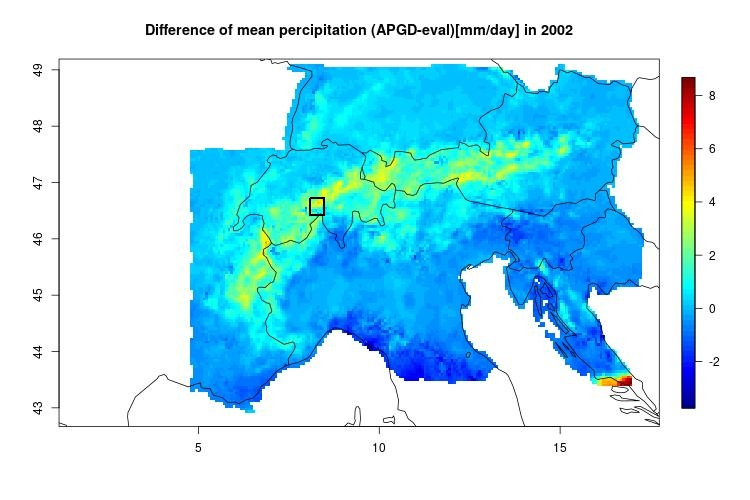
\includegraphics[width=\textwidth]{mean_n/2002dif_mprs_alp3eval-apgd.jpg}
			\caption{Evaluation, ALP-3}
			\label{fig:dif_mean_2002:alp3_eval}
		\end{subfigure}
	\caption{Differenzen des jährlichen Mittels über den Niederschlag im Jahr 2002}
	\label{fig:dif_mean_2002}
\end{figure}

Wie in den Grafiken bei Abb.\ref{fig:dif_mean_2002} zu erkennen ist bleibt in einem gewissen Bereich die Abweichungen über alle Datensätze am größten. Deshalb wurde dieser in Folge gesondert betrachtet. Der Bereich wurde in den Abbildungen gekennzeichnet.\\
Diese gekennzeichnete Fläche wurde aus allen Datensätzen ausgeschnitten und im Jahr 2002 über dessen Fläche gemittelt, somit ergab sich aus dem Rechteck ein Mittelwert für jeden Tag für jeden Datensatz. Von diesen Werten wurden dann die ebenfalls Flächen-gemittelten Beobachtungsdaten (APGD) abgezogen und im Diagramm in Abb.\ref{fig:diff_2002} gegen die Zeit aufgetragen.\\
\begin{figure}[h]
	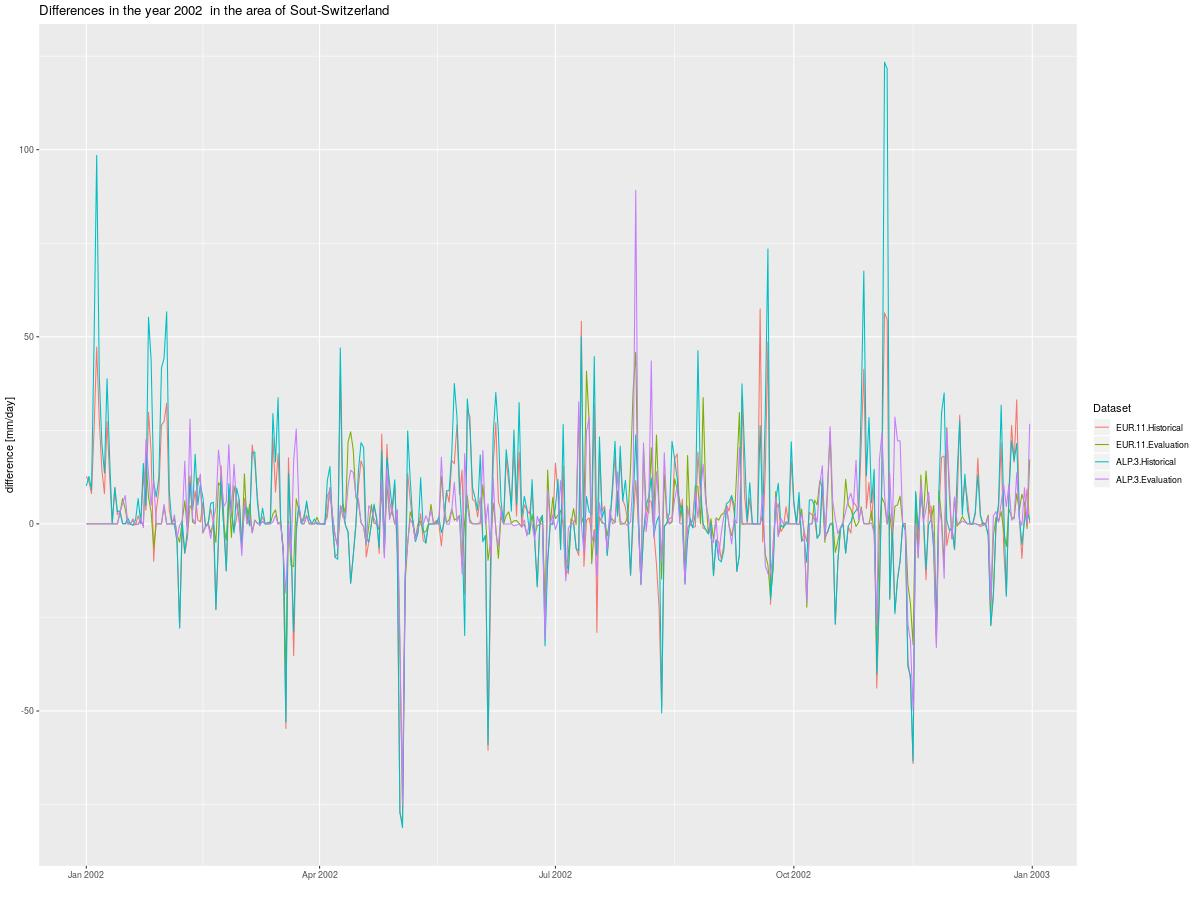
\includegraphics[width=0.95\textwidth]{mean_n/differences_2002.jpg}
	\caption{Die Differenzen für den in der Abb. \ref{fig:dif_mean_2002} gekennzeichneten Bereich im Jahr 2002. Es muss beachtet werden, dass hier die tägliche Inkonsistenz betrachtet wird, dies ist nicht ein Fehler des Modells.}
	\label{fig:diff_2002}
\end{figure}\\
Man sieht in Abb.\ref{fig:diff_2002}, dass die Abweichungen über das Jahr verteilt stark fluktuieren. Beachtenswert ist dabei, dass die Ausschläge der Kurven für den ALP-3 Datensatz deutlich größer und auffallend in das Positive verschoben sind. Die Kurvenform der beiden, Historical und Evaluation Datensätzen sind nahezu identisch, was auf Fehler in den Antriebsdaten zurückzuführen ist. Da die Ausschläge gemittelt über das ganze Gebiet (vgl. Abb.\ref{fig:mean_boxplots} und Abb.\ref{fig:mean_freq_plots}) für den ALP-3 Datensatz deutlich besser sind ist es in diesem gesondert betrachteten Gebiet wahrscheinlich zu einem Overfitting des Modells gekommen und die extremen Ausschläge sind Fluktuationen die daraus resultieren. Um die Ergebnisse der beiden RCM's EUR-11 und ALP-3 besser untersuchen zu können wurden die zwei Datensätze mit den größten Abweichungen (Historical aus EUR-11 und ALP-3) in Abb.\ref{fig:precip_2002} dargestellt.\\

\begin{figure}[b]
	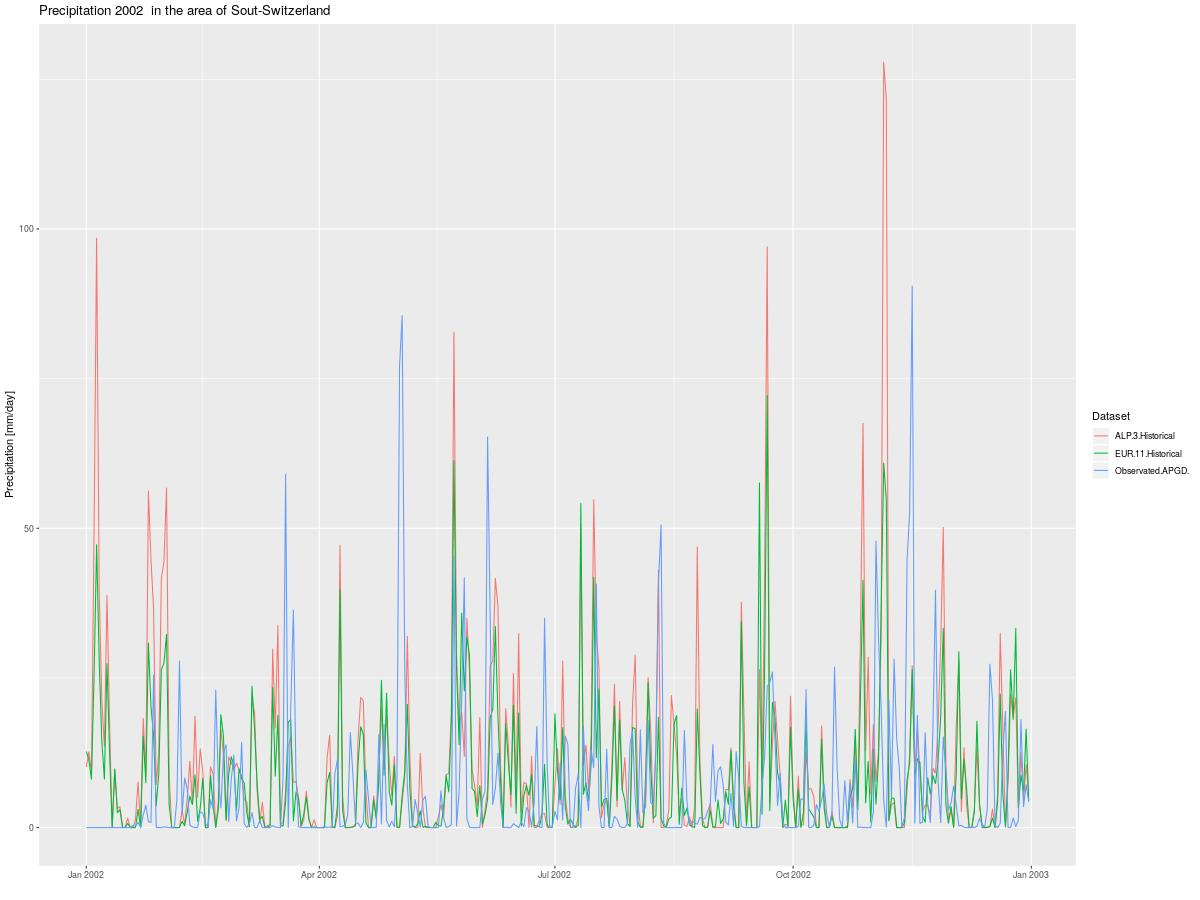
\includegraphics[width=0.90\textwidth]{mean_n/historical_2002.jpg}
	\caption{Niederschlag im Jahr 2002 für den in Abb.\ref{fig:dif_mean_2002} gekennzeichneten Bereich aus den Datensätzen Historical von ALP-3 bzw. EUR-11 gegen die Beobachtungsdaten aus APGD}
	\label{fig:precip_2002}
\end{figure}
\begin{figure}[b]
	\begin{subfigure}{0.49\textwidth}
		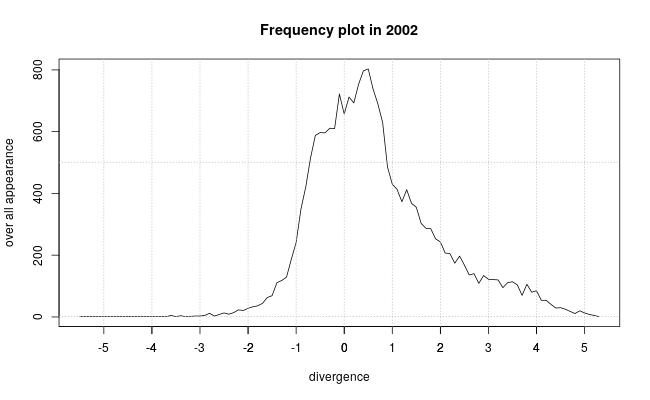
\includegraphics[width=\textwidth]{mean_n/2002frequenciesdif_mprs_hist-obs.jpg}
		\caption{EUR-11, Historical}
	\end{subfigure}
	\begin{subfigure}{0.49\textwidth}
		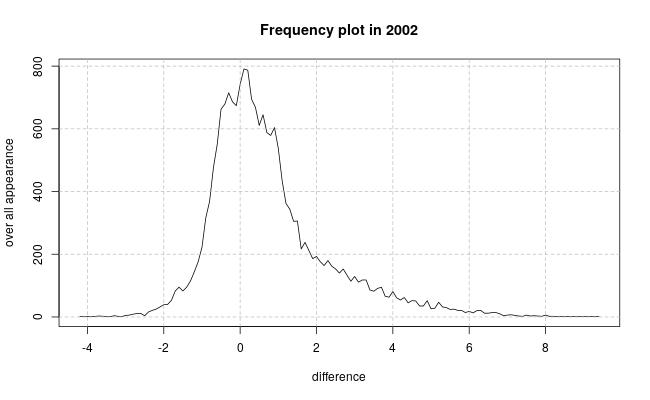
\includegraphics[width=\textwidth]{mean_n/2002frequenciesdif_mprs_alp3hist-apgd.jpg}
		\caption{ALP-3, Historical}
	\end{subfigure}
	\begin{subfigure}{0.49\textwidth}
		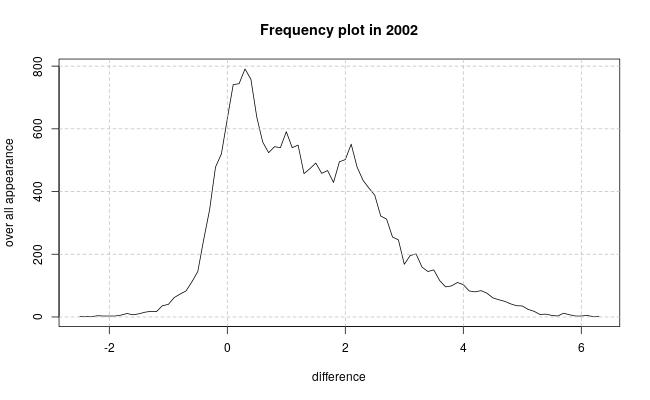
\includegraphics[width=\textwidth]{mean_n/2002frequenciesdif_mprs_eval-obs.jpg}
		\caption{EUR-11,Evaluation}
	\end{subfigure}
	\begin{subfigure}{0.49\textwidth}
		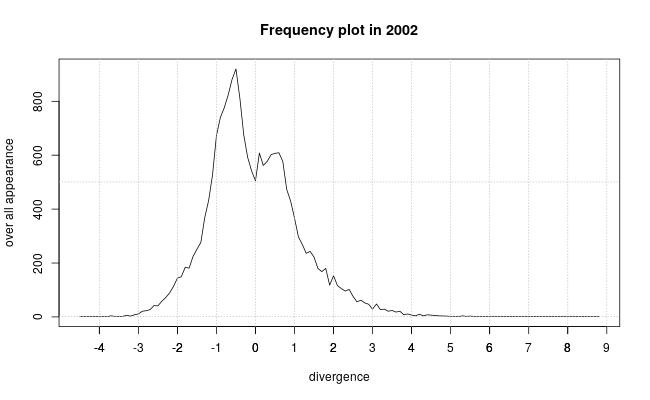
\includegraphics[width=\textwidth]{mean_n/2002frequenciesdif_mprs_alp3eval-apgd.jpg}
		\caption{ALP-3, Evaluation}
	\end{subfigure}
	\caption{Häufigkeit gewisser Abweichungen für das gemittelte Jahr 2002 in den beiden Historical - Datensätzen (betrachtetes Gebiet: \underline{gesamter} Alpenraum)}
	\label{fig:freq_2002}
\end{figure}

In der Abb. \ref{fig:precip_2002} liegen die im regionalen Klimamodell (ALP-3) die vorhergesagten Niederschlagsmengen für größere Niederschlagsmengen z.B. im Mai 2002 um einiges näher an den beobachteten Daten. Es werden jedoch auch manche Niederschlagsereignisse schlichtweg überschätzt, was sich dann im Gesamtbild schlecht auswirkt (vgl.\ref{fig:freq_2002}: die Kurve ist deutlich ins Positive verschoben.\\
Das Klimamodell welches die Konvektion nicht simuliert (EUR-11) scheint dauernd eine gewisse Fluktuation im Niederschlag zu errechnen, ohne gezielt Starkregenereignisse zu reproduzieren. Dies ist gut im Bereich April 2002 in der Abb. \ref{fig:precip_2002} zu erkennen: Die Fluktuationen scheinen gewissermaßen ständig aufzutreten. Das ist auf die Parametrisierung der Konvektion zurückzuführen. Da dadurch auch keine längeren Regenpausen vorkommen können, ist dies ein großes Manko in der Vorhersagekraft von diesen Modellen für die zukünftige Entwicklung des Klimas auf regionaler Ebene (siehe ''Bias Correction, Quantile Mapping, and Downscaling: Revisiting the Inflation Issue'' von D.Maraun \cite{biasMaraun}). \\
Das Konvektion-simulierende Klimamodell ALP-3 scheint besonders im Winter und im Herbst Niederschlagsextrema zu überschätzen. Im Sommer  bzw. Frühling stimmen die Daten relativ gut überein. Manche Extrema sind zwar zeitlich verschoben, jedoch muss bemerkt werden, dass die historischen Tage nichts mit den simulierten Tage im Klimamodell gemein haben, somit darf die zeitliche Verteilung nicht zu genau genommen werden. Sondern es muss eine gewisse Toleranz, wann ein Starkregenereignis eintritt mit-einberechnet werden.\\
\end{comment}
\section{Zusammenfassung}\label{sec:zusammenfassung_01}
Wie in diesem Kapitel gezeigt wurde, liegen die Abweichungen der Mittelwerte beider regionalen Klimamodell ähnlich verteilt vor. Dies kann darauf zurückgeführt werden, dass das feinere RCM CCLM5-0-9 in das gröber genested wurde. Die beiden Datensätze (ALP3 und EUR11) unterscheiden sich besonders in den Ausreißern (vgl. Abb \ref{fig:mean_boxplots}), das feinere RCM hat viel stärkere maximale Abweichungen als das gröbere. Dies ist auf das noch mangelhafte tuning des jüngeren und feineren Modells zurückzuführen.\\
Durch das Mitteln der Daten wurden die Extremniederschläge aus den Daten ''wekgemittelt'' und da der Mittelwert des Niederschlags nicht das Klima einer Region beschreibt kann der Mittelwert nicht zur vollständigen Evaluation eines Modells herangezogen werden. Nichtsdestotrotz gibt der Mittelwert einen guten Aufschluss darüber, wo die größten Abweichungen herrschen (siehe Abbildung \ref{fig:mean_diff}). Will man eine einzelne Region über eine Jahreszeit oder auch die gesamte Zeitspanne genauer betrachten, steht man vor dem Problem, dass die simulierten Tage nicht direkt mit den historischen Tagen in Verbindung gebracht werden dürfen(vgl. Kapitel \ref{chap:modells}). Um nun diese tägliche Inkonsistenz aus der Evaluierung Außenvorzulassen soll im nächsten Kapitel auf die alljährlichen Extremniederschläge über das 99.Quantil eingegangen werden, wodurch diese Inkonsistenz in den Kalendertagen umgangen wird: Es wird nicht der Tag X in den Beobachtungsdaten mit dem Tag X in den Modelldaten verglichen sondern der Tag mit dem höchsten Niederschlag bzw. dem 99.Quantil des Niederschlag in beiden Datensätzen.
\section{R-Code}
\begin{lstlisting}[language=R]
	observation <- stackAPGD(getAPGD())
	mean_observations<-getAnnualMeanObs(observation)
	mean_mean_observations<-calc(mean_observations, fun=mean)
	eval_eur11 <- stackSim(getEUR11regridded_eval_pr(), varname = "pr", factor = 3600*24) # factor for the precipitation-unit
	mean_eval_eur11<-getAnnualMeanSim(eval_eur11) # calculates the annual mean and places it in a raster (=>10years==10layers)
	mean_mean_eval_eur11 <- calc(mean_eval_eur11, fun=mean) #calculate the mean over all years
	extent(mean_mean_observations)<-extent(mean_mean_eval_eur11) # for better representation
	dif_mean_eval_eur11<-overlay(mean_mean_eval_eur11, mean_mean_observations,fun=function(x,y){return((x - y))}) #subtract each grid-cell
\end{lstlisting}
Ein Ausschnitt des Codes, der für die Berechnungen des Mittelwertes und der Differenzen verwendet wurde. Die Funktionen getAPGD() und getEUR11regrid\_eval\_pr() liefert eine liste der Dateien mit den Daten zurück. Die beiden Funktionen stackSim() und stackAPGD() legen die Daten in eine Liste aus rastern ab. danach wird über die einzelnen Elemente der Liste der Mittelwert und in Folge der Mittelwert aller Mittelwerte berechnet (stets für jede Zelle einzeln). Diese Mittelwerte werden voneinander abgezogen (Modell - Beobachtung).
	
	
	\chapter{Conclusion}
	Die einzelnen Modelldaten unterscheiden sich am stärksten durch die beiden unterschiedlichen globalen Klimamodelle (GCM's) mit denen sie betrieben wurden. Die Ergebnisse, welche durch das Betreiben mit den Re-Analysedaten erhalten wurden, waren viel näher an den Beobachtungsdaten als jene, welche durch das MPI-ESM-LR erhalten wurden. Was aber weiter nicht verwunderlich ist, da zweiteres ein in die Vergangenheit gerechnetes GCM ist und deshalb z.B. Extremwetterlagen nicht leicht bzw. nicht zeitlich korrekt abbilden kann.\vspace{7pt}\\

Die im Kapitel \ref{chap:mean} erhaltenen Ergebnissen deuten darauf hin, dass das regionale Klimamodell im Mittel eine bessere Vorhersage gewähren, solange das GCM die tatsächlichen Gegebenheiten korrekt abbildet. Das RCM betrieben mit den Re-Analysedaten gibt mit dynamisch simulierter Konvektion (ALP-3) eine weitaus besseren \textbf{mittlere} Abweichung als das RCM mit parametrisierter Konvektion. Mit dem GCM MPI-ESM-LR betrieben ergibt sich jedoch eine leicht größere mittlere Abweichung des Biases (vgl. Abb.\ref{fig:yearly_mean_biases}) für den ALP-3 Datensatz.\\
Vergleicht man die Streuung der mittleren Abweichungen scheint durch die parametrisierte Konvektion weniger starke Ausreißer erzeugt zu werden, wie in der Abb.\ref{fig:mean_boxplots} zu erkennen ist. Daraus kann geschlossen werden, dass im Mittel die parametrisierte Konvektion ausreichend ist um ein GCM auf regionalen Maßstab herunterzubrechen.\vspace{7pt}\\

Wenn man die jährliche mittlere Abweichung eines Jahres betrachtet (Kapitel \ref{section:2002}) so ergeben sich leicht abweichende Aussagen über die unterschiedlichen Datensätze als für das Mittel eines Jahrzehnts: Die Streuung scheint zwar immer noch durch die dynamisch simulierte Konvektion stärker zu sein (vgl. Abb.\ref{fig:freq_2002}), Die Verteilungskurven der Häufigkeiten sind jedoch spitzer zulaufend über 0, was einer geringeren Abweichung im Mittel entspricht. Dies kann auch durch die in Tabelle \ref{tab:appendix} angegebenen mittleren Abweichungen nachvollzogen werden.\vspace{7pt}\\

Die Modellierung von Starkniederschläge, betrachtet über das ganze Jahr scheint die parametrisierte Konvektion am besten zu bewerkstelligen. Wieder ist dies stark davon abhängig, wie gut das GCM die Wirklichkeit abbildet, mit welchem das RCM betrieben wird. Dazu ist die Darstellung der Boxplots in Abb.\ref{fig:quantile_all_boxplots} ein maßgebliches Argument: Die Ausreißer scheinen zwar wieder für die parametrisierte Konvektion in einem engeren Rahmen zu liegen jedoch ist der mittlere Bias des 99. Quantils für die simulierte Konvektion betrieben mit den Re-Analysedaten um näher bei 0.\\
Diese Abweichungen finden sich vor allem in gebirgigen Gebieten am Alpenhauptkamm und  Gebieten mit komplexen Wettersystemen wie z.B. Genua (siehe Abb.\ref{fig:quantile_alp3}). Dies lässt darauf schließen, dass in solchen Gebieten die Simulation der Konvektion noch nicht ausgereift bzw. vollends durch das Modell erfasst wurde. Da besonders in diesen Regionen die simulierte Konvektion bessere Ergebnisse bringen sollte, wie D.Maraun et al. in \cite{maraun_value} postuliert.\vspace{7pt}\\

Für die Starkregenereignisse (99. Quantil des Niederschlags) in den einzelnen Jahreszeiten scheint sich das Muster der Abweichung etwas anders abzuzeichnen als in den bisherigen Betrachtungen:\\
Im Frühling dominiert die Modellierung mit parametrisierter Konvektion durch ihre geringe Streuung und den guten Bias, betrieben mit den Re-Analysedaten. Für die Ansteuerung des RCM's mit dem MPI-ESM-LR scheinen sich die Ausreißer durch die simulierte Konvektion besser abzubilden bzw. ist die Abweichung näher bei 0. Der Datensatz Evaluation ALP-3 sticht durch seine extremen Ausreißer hervor, was auf ein bestimmtes Gebiet im Süden Kroatiens zurückzuführen ist (vgl. Abb.\ref{fig:seasons_boxplots}). Beachtenswert ist, dass dieses Gebiet nur im Sommer keine so extremen Ausreißer produziert wie in allen anderen Jahreszeiten. Da das Gebiet am Rande des Gitters liegt, könnte es sich auch um eine Fehlabbildung im Datensatz handeln. Betrachtet man kleinere Gebiete und deren Flächen-gemittelten Niederschlag, scheint sich für die Extremniederschläge im Frühling ein weitaus besseres bzw. Beobachtungs-näheres Muster abzubilden: vgl. Abb.\ref{fig:seasons:pr_over_undersim_eval_alp3} mit Abb.\ref{fig:seasons:hist_eur11:overundersim_mean}. Die Niederschläge bezogen auf den Durchschnittsniederschlag kommen den beobachteten Daten am nächsten mit der simulierten Konvektion.\\
Im Sommer streuen sich die Abweichungen der Daten aus dem RCM mit simulierter Konvektion am wenigsten, da sich in dieser Jahreszeit die Konvektion am stärksten abzeichnet bzw. die stärksten Auswirkungen auf den Niederschlag haben, ist dies eine Bestätigung der Vorhersagequalität des RCM's. Der Bias liegt zwar für den Historical-ALP3 Datensatz etwas über dem des EUR-11 Datensatzes aber wenn die Streuung mit berücksichtigt wird, ist für den Sommer die Vorhersage von Starkregenereignissen durch das RCM mit dynamisch simulierter Konvektion am besten gegeben. Dies fällt auch besonders gut auf, wenn der Niederschlag gegen den mittleren Niederschlag einer Fläche aufgetragen wird. Das Muster des Niederschlags folgt um einiges besser den Beobachtungsdaten, wenn die Konvektion simuliert und nicht nur parametrisiert ist: Die Ausschläge von Niederschlagsextrema sind durch die parametrisierte Konvektion eine nahezu Vorhersagbare Frequenz, durch die simulierte Konvektion den Beobachtungsdaten treu (vgl. Abb.\ref{fig:seasons:undersim_eval_eur11} mit Abb.\ref{fig:seasons:mean_alp3}).
Winter und Herbst wurden nicht gesondert betrachtet, doch in diesen Jahreszeiten zeichnet sich die Abweichung der Starkregenereignisse fast gleich ab wie im Frühling. Dies ist besonders gut in der Grafik \ref{fig:seasons_boxplots} zu erkennen. Beachtenswert dabei ist, dass der Bias des Datensatzes Historical EUR-11 im Herbst und des Datensatzes Evaluation EUR-11 im Winter das Minimum bildet. Des Weiteren muss in Betracht gezogen werden, dass die Abweichungen im Winter besonders schlecht für das RCM mit simulierter Konvektion ausfällt, da die Streuung und der Bias für beide Datensätze, Evaluation und Historical weit über dem Bias der Datensätze aus dem RCM mit parametrisierter Konvektion liegt.\\
Abschließend kann gesagt werden, dass das RCM mit simulierter Konvektion im Schnitt schlechter abschneidet als jenes mit parametrisierter Konvektion aber die Frequenz der Niederschläge bzw. Extremausschläge besser dargestellt werden.
	
	\appendix
	\chapter{Appendix Title}
	\begin{table}[h!]
	\begin{tabularx}{\textwidth}{X|X|X|X|X|}
		\cline{2-5}
		& \textbf{Historical EUR-11} & \textbf{Evaluation EUR-11}& \textbf{Historical ALP-3} & \textbf{Evaluation ALP-3}\\
		\hline
		Jahrzehnt-Mittel, BIAS& $1.4743$ & $0.21764$ & $1.55835$ & \cellcolor{YellowGreen}$0.17723$\\
		\cline{2-5} \& Streuung& $[-2.7...6.0]$ & \cellcolor{YellowGreen}$[-4.6...3.9]$ &$[-2.5...12.2]$& $[-3.7...8.7]$\\
		\hline\hline
		Jahresmittel (2002), BIAS & $0.66826093$ & $1.34588$ & $0.7579549$&\cellcolor{YellowGreen}$-0.03313489$\\
		\cline{2-5}\& Streuung & $[-5.45...5.28]$ & \cellcolor{YellowGreen}$[-6.18...4.44]$ &$[-4.17...9.38]$& $[4.46...8.79]$\\
		\hline\hline
		99. Quantil& $2.50113$ & $-2.865$ & $5.35387$&\cellcolor{YellowGreen}$2.35926$\\
		\cline{2-5} des Jahrzehnts, BIAS \& Streuung& $[-54.53...43.28]$ &[-62.85... 32.21] &\cellcolor{YellowGreen}[-35.94... 54.15]& [-45.48... 260.78]\\
		\cline{5-5}
		&&&\cellcolor{YellowGreen}&[-45.48... 46.45]* \\
		\hline\hline
		99. Quantil Frühling, BIAS& $5.36773$ & $\cellcolor{YellowGreen}1.71555$ & $8.86566$&$7.01032$\\
		\cline{2-5} \& Streuung	& [-77.04... 43.64] & \cellcolor{YellowGreen}[-77.28... 39.27] & [-52.06... 64.85] & [-38.64... 294.38]\\
		\cline{5-5}&&&&\cellcolor{YellowGreen}[-38.7...52.3]*\\
		\hline
		99. Quantil Sommer, BIAS & $5.32457$ & $-5.33069$ & $6.68616$&\cellcolor{YellowGreen}$-2.6092$\\
		\cline{2-5}  \& Streuung & [-54.59... 64.22] & [-68.84... 35.13] & \cellcolor{YellowGreen}[-41.92... 59.33] & [-66.31... 59.62]\\
		\hline
		99. Quantil Herbst, BIAS & \cellcolor{YellowGreen}$0.9993$ & $-4.28896$ & $3.07413$&$3.16922$\\
		\cline{2-5}\& Streuung& [-96.62... 60.89]& [-79.95... 70.3] & \cellcolor{YellowGreen}[-65.85... 80.49]& [-57.39... 414.30]\\
		\cline{5-5}&&&&[57.57... 96.0]*\\
		\hline
		99. Quantil Winter, BIAS& \cellcolor{YellowGreen}$4.06577$ & $-0.13379$ & $8.33802$&$5.2272$\\
		\cline{2-5}\& Streuung & [-60.08... 41.26] & \cellcolor{YellowGreen}[-74.79... 31.48] & [-48.56... 82.45] & [-57.17... 529.50]\\
		\cline{5-5}&&&&[-57.93..55.9]*\\
		\hline
	\end{tabularx}
	\caption{Zusammenfassende Tabelle aller Berechnungen, mit gekennzeichneten besten Ergebnissen in grün ([*]ohne Ausreißer-Bereich bei Kroatien)}
	\label{tab:appendix}
\end{table}
	\printbibliography
\end{document}
